Consider an implicit closed curve in 2D

$$f(x,y)=0$$

given by a parametrization $x=x(t), y=y(t), t\in[0,L]$. For a choice of parameter values
$\{t_j\}=\{t_1,\ldots,t_N\}$ consider the point cloud $\textbf{x}_j=(x_j,y_j)=(x(t_j),y(t_j))$. The goal
of this exercise is to reconstruct the implicit function from the given point cloud.\\

Step 1: Find an outer normal vector $\textbf{n}_j$ to the curve at each point $\{\textbf{x}_j\}$.\\

Step 2: Fix $\alpha>0$ small and comnsider the inner and outer positions

$$\textbf{x}_j^-=\textbf{x}_j-\alpha\textbf{n}_j,\;\;\textbf{x}_j^+=\textbf{x}_j+\alpha\textbf{n}_j$$

Step 3: Interpolate the $3N$ data points
$(\textbf{x}_j^-,-\alpha),(\textbf{x}_j,0),(\textbf{x}_j^+,\alpha)$ using RBF interpolants. That is find
a function $F:\mathbb{R}^2\to\mathbb{R}$,

$$F(\bf{x})=\sum_{j=1}^Nc_j\phi(||x-x_j||)$$

such that $F(\bf{x}_j)=0$ and $F(\bf{x}_j^-)=-\alpha,\;F(\bf{x}_j^+)=\alpha$.\\

Step 4: Restrict $F$ to the level set $F(x,y)=0$ to obtain the RBF interpolation for the implicit curve
$f(x,y)=0$\\\\

\begin{solution}\renewcommand{\qedsymbol}{}\ \\
    For this problem we will be trying to interpolate a nephroid curve. This is given by the parametric
    equations

    $$x(t) = 0.5(3\cos(t)-\cos(3t))$$

    $$y(t) = 0.5(3\sin(t)-\sin(3t))$$

    for $0\leq t\leq2\pi$. So, using the code that we built in class on the following point cloud in 2D,
    we get the following 3D extrusion and then the following level curve. As we can see, the level curve
    is not quite exact. This is due to the cusps on the original curve affecting the normal vectors.
    However, the level curve does do a fairly good job of interpolating.
    
    \begin{center}

        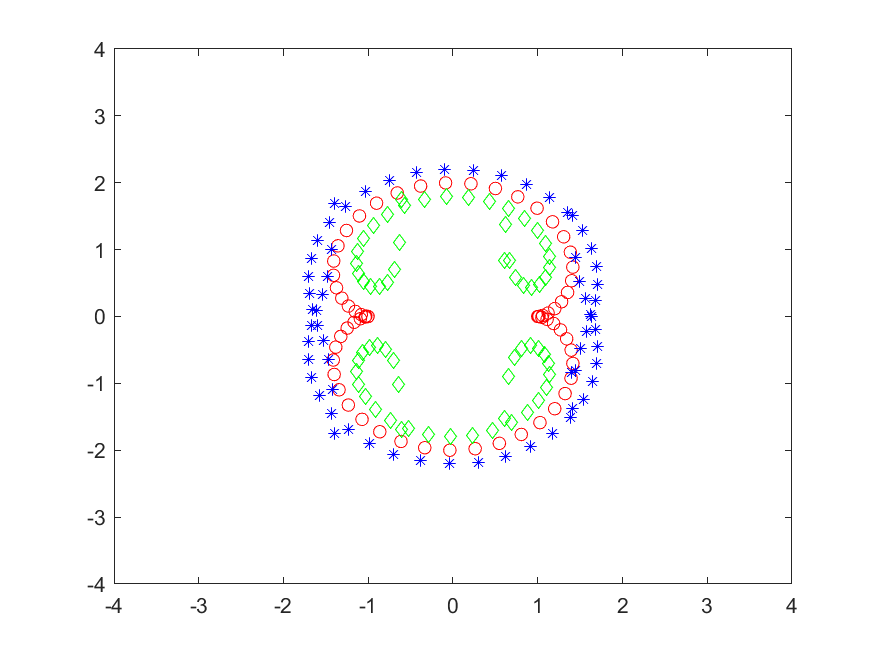
\includegraphics[scale=0.69]{problem1norm.PNG}
        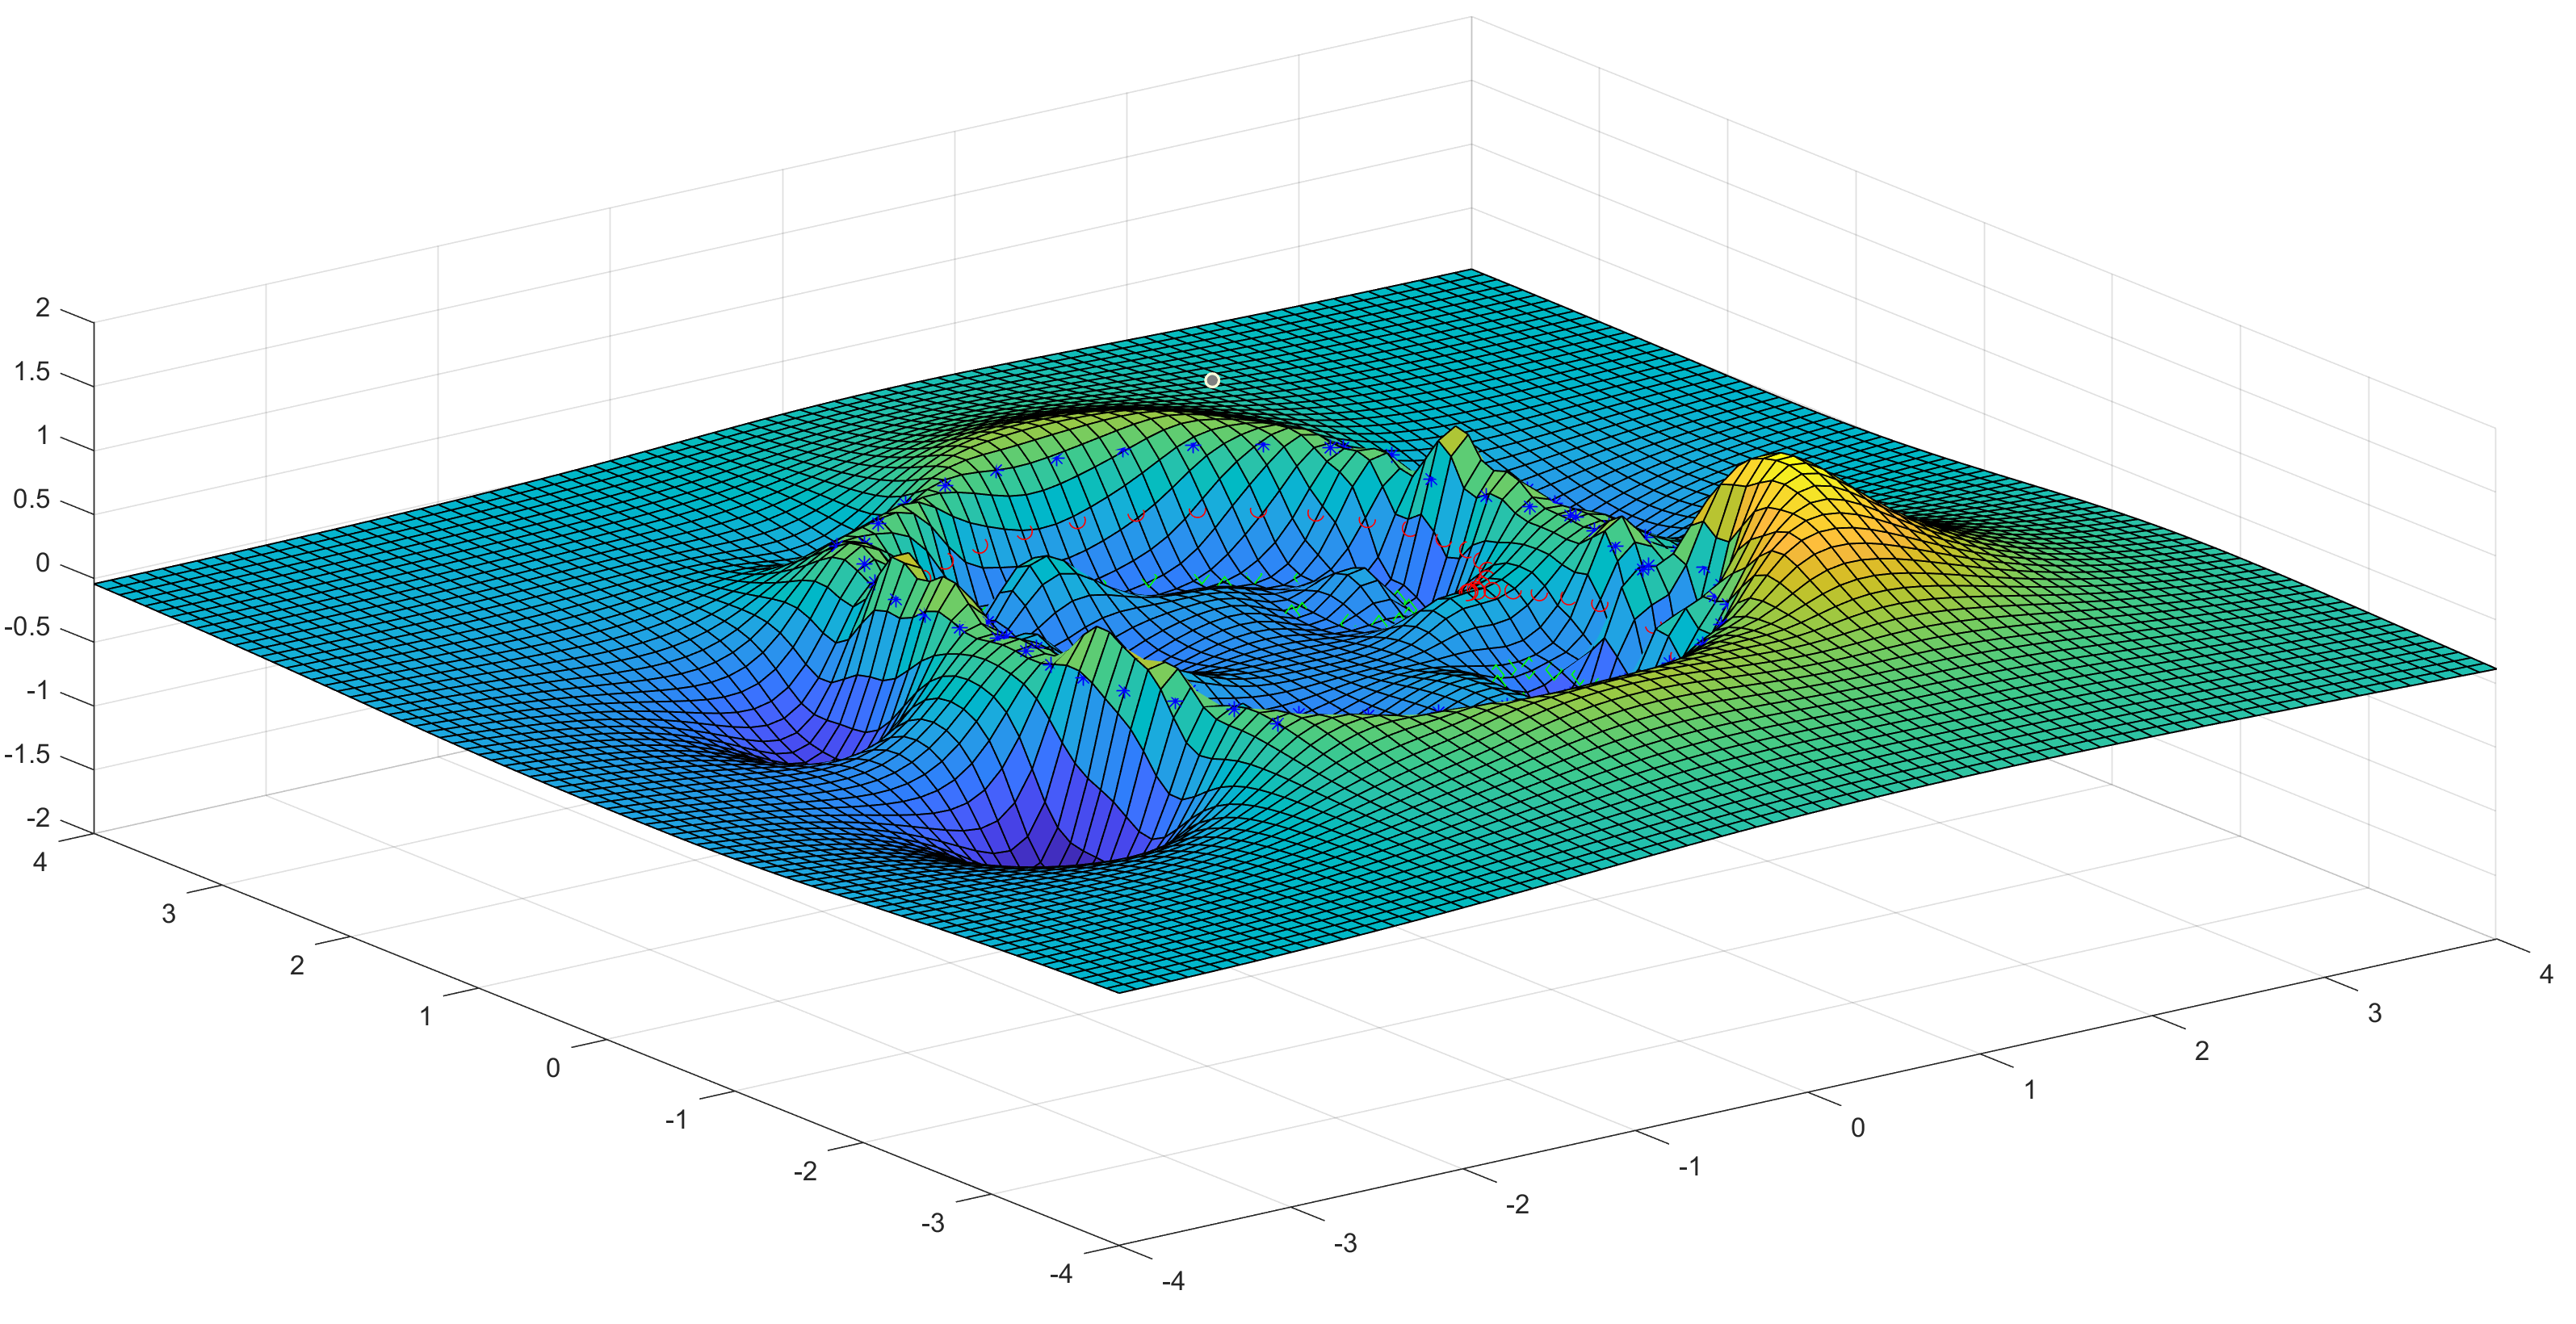
\includegraphics[scale=0.15]{problem1ext.PNG}
        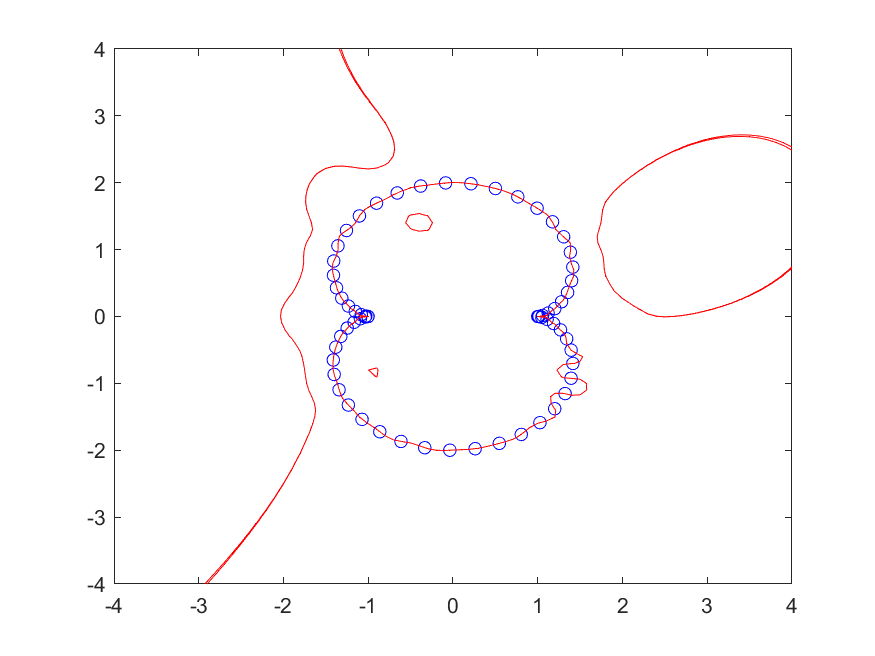
\includegraphics[scale=0.69]{problem1lvl.PNG}

    \end{center}

\end{solution}

\newpage
\lstinputlisting{problem1.m}